\ac{MUTE} prend la forme d'une application web qui permet de créer et de gérer des documents textes.
Chaque document se voit attribuer un identifiant, supposé unique.
L'utilisateur-rice peut alors ouvrir et partager un document à partir de son URL.

L'application permet à l'utilisateur-rice d'être mis-e en relation avec les autres pairs actuellement connectés qui travaillent sur ce même document.
Pour cela, l'application utilise le protocole WebRTC afin d'établir des connexions \ac{P2P} avec ces derniers.
Une fois les connexions \ac{P2P} établies, le service fourni par le système pour mettre en relation les pairs n'est plus nécessaire.

Une fois connecté à un autre pair, l'utilisateur-rice récupère automatiquement les modifications effectuées par ses pairs de façon à obtenir la version courante du document.
Iel peut alors modifier le document, \ie ajouter, supprimer du contenu ou encore modifier son titre.
Ses modifications sont partagées en temps réel aux autres pairs connectés.
À la réception de modifications, celles-ci sont intégrées à la copie locale du document.
\autoref{fig:interface-mute-editor} illustre l'interface utilisateur de l'éditeur de document de MUTE.
\begin{figure}[!ht]
    \centering
    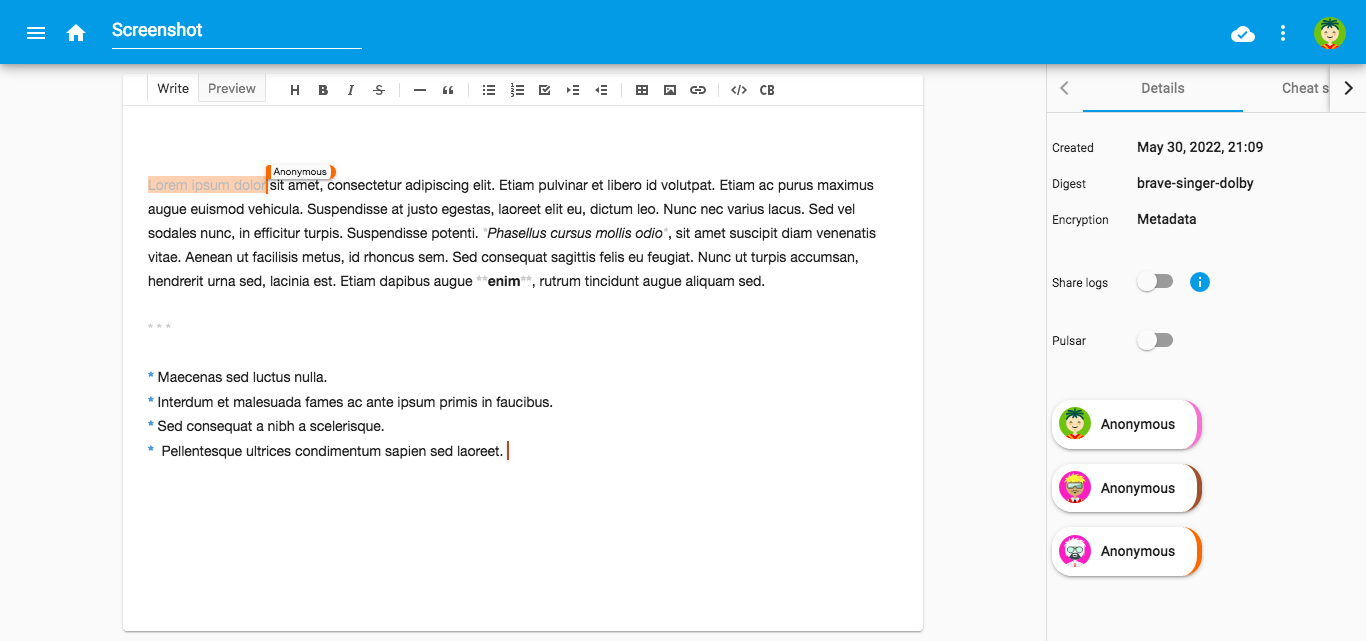
\includegraphics[width=\linewidth]{img/screenshot-mute-editor.png}
    \caption{Capture d'écran d'une session d'édition collaborative avec MUTE}
    \label{fig:interface-mute-editor}
\end{figure}

Pour garantir la confidentialité des échanges, \ac{MUTE} utilise un protocole de génération de clés de groupe.
Ce protocole permet d'établir une clé de chiffrement connue seulement des pairs actuellement connectés, qui est ensuite utilisée pour chiffrer les messages entre pairs.
Ce protocole permet de garantir les propriétés de \emph{backward secrecy} et de \emph{forward secrecy}.
\begin{definition}[Backward Secrecy]
    \label{def:backward-secrecy}
    La \emph{Backward Secrecy} est une propriété de sécurité garantissant qu'un nouveau noeud ne pourra pas déchiffrer avec la nouvelle clé de chiffrement les anciens messages chiffrés avec une clé de chiffrement précédente.
\end{definition}
\begin{definition}[Forward Secrecy]
    \label{def:forward-secrecy}
    La \emph{Forward Secrecy} est une propriété de sécurité garantissant qu'un nouveau noeud ne pourra pas déchiffrer avec la nouvelle clé de chiffrement les futurs messages chiffrés avec une prochaine clé de chiffrement.
\end{definition}

Une copie locale du document est sauvegardée dans le navigateur, avec l'ensemble des modifications.
L'utilisateur-rice peut ainsi accéder à ses documents même sans connexion internet, pour les consulter ou modifier.
Les modifications effectuées dans ce mode hors-ligne seront partagées aux collaborateur-rices à la prochaine connexion de l'utilisateur-rice.

Finalement, la page d'accueil de l'application permet aussi de lister ses documents.
L'utilisateur-rice peut ainsi facilement parcourir ses documents, récupérer leur url pour les partager ou encore supprimer leur copie locale.
\autoref{fig:interface-mute-document-list} illustre cette page de l'application.
\begin{figure}[!ht]
    \centering
    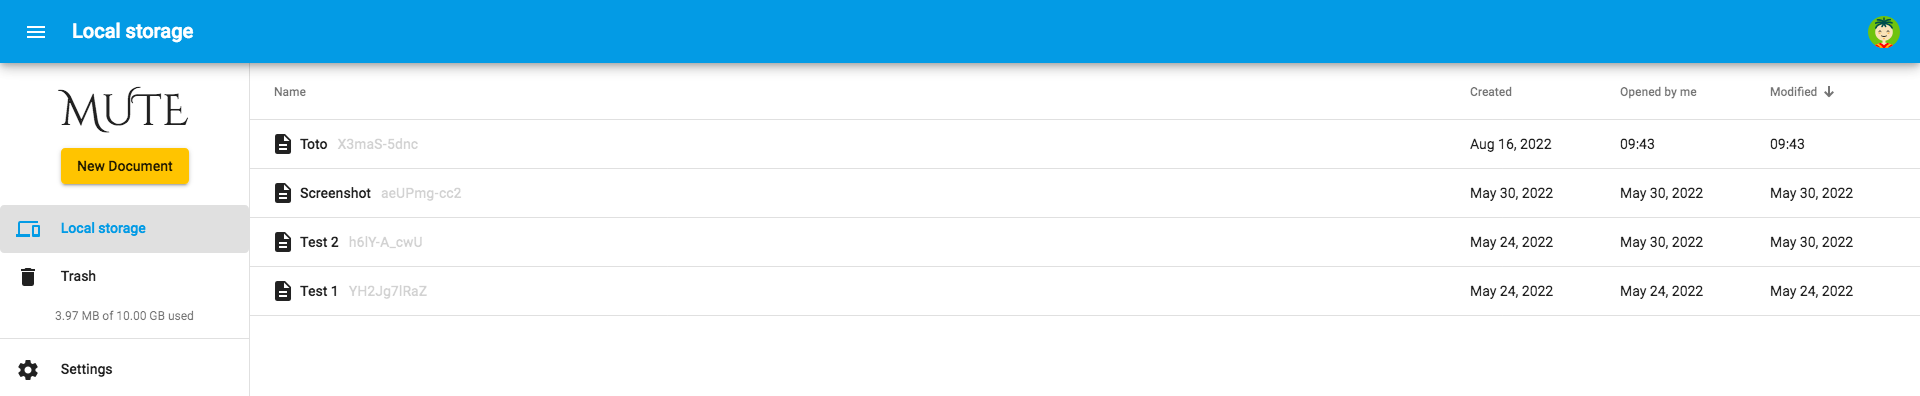
\includegraphics[width=\linewidth]{img/screenshot-mute-document-list.png}
    \caption{Capture d'écran de la liste des documents.}
    \label{fig:interface-mute-document-list}
\end{figure}
